\documentclass[listof=totoc,DIV11,a4paper]{scrreprt}

\usepackage[utf8]{inputenc}
\usepackage[T1]{fontenc}
\usepackage[ngerman]{babel}

\usepackage[hidelinks]{hyperref}
\usepackage{color}
\usepackage{graphicx}
\usepackage[onehalfspacing]{setspace}
\usepackage{listings}

% Listings-Einstellungen
\lstset{basicstyle=\footnotesize, captionpos=b, breaklines=true, showstringspaces=false, tabsize=2, frame=lines, numbers=left, numberstyle=\tiny, xleftmargin=2em, framexleftmargin=2em}
\makeatletter
\def\l@lstlisting#1#2{\@dottedtocline{1}{0em}{2em}{\hspace{1,5em} Lst. #1}{#2}}
\makeatother

\newcommand{\od}{O\textunderscore DIRECT }

\title{Systemnahes Programmieren -- Dokumentation}
\subtitle{Hochschule Karlsruhe -- Technik und Wirtschaft}
\author{Richard Gottschalk, 40365 \and Tobias Harms, 42894}
\date{Sommersemester 2015}

\begin{document}
\begin{singlespace}
\maketitle
\tableofcontents
\listoffigures
\lstlistoflistings
\end{singlespace}
\chapter{Einführung}
Im Labor \glqq Systemnahes Programmieren\grqq\ geht es darum einen Compiler zu programmieren, welcher aus einer gegebenen Grammatik einen Assembler-ähnlichen Code erzeugt. Für diesen Code gibt es einen Interpreter, sodass die Programme dann tatsächlich ausgeführt werden können.

\begin{figure}[h]
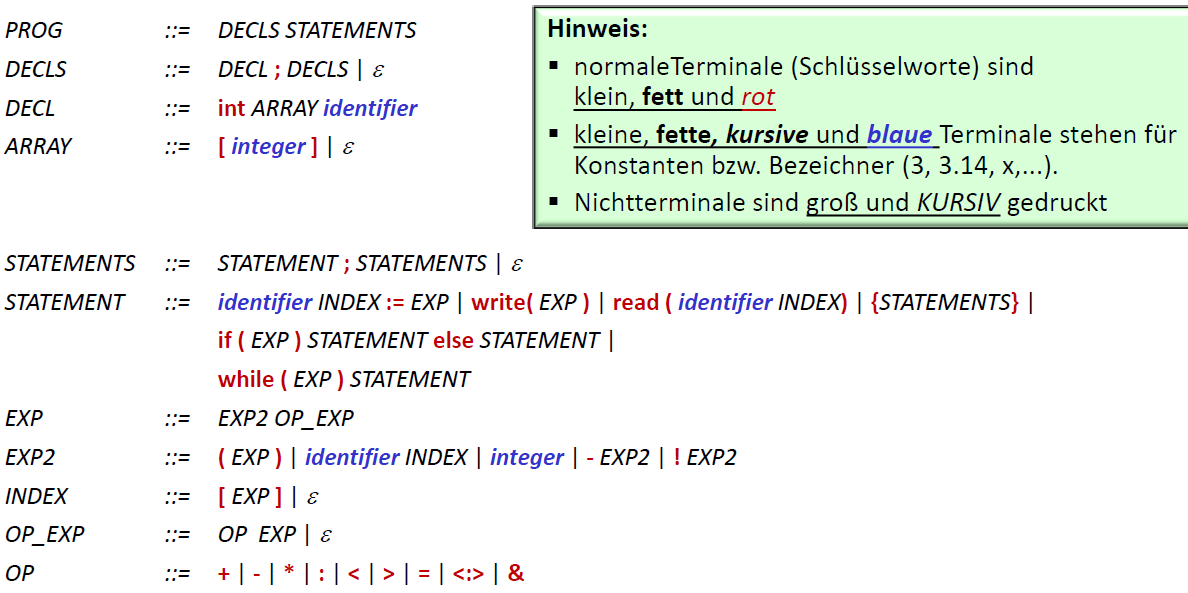
\includegraphics[width=\linewidth]{images/grammatik}
\label{img:grammatik}
\caption{Die Grammatik der zu erkennenden Sprache}
\end{figure}

Für diese Aufgabe waren einige Voraussetzungen gegeben:
\begin{itemize}
\item Die Verwendung von Linux
\item Programmieren in C++
\item Die Verwendung von GNU make zum Build-Management
\item Die Verwendung von \od und posix\textunderscore memalign beim Buffer (siehe Kap. \ref{subsec:odirect}) 
\end{itemize}

Die Aufgabe wurde in zwei Aufgabenteile zerlegt, den \emph{Scanner} (Kapitel \ref{kap:scanner}) und den \emph{Parser} (Kapitel \ref{kap:parser}).

\chapter{Scanner}\label{kap:scanner}
Der Programmteil \emph{Scanner} zerlegt den Quellcode in Tokens, welche dann vom Parser weiter verarbeitet werden. Der Scanner muss sich also um das Einlesen aus der Quelldatei (Buffer, siehe Kapitel \ref{sec:buffer}), die Erkennung von Tokens (Automat, siehe Kapitel \ref{sec:automat}) und die Speicherung von Identifiern (Symboltabelle, siehe Kapitel \ref{sec:symtable}) kümmern. Die Aufgabe des Scanners ist also die \emph{lexikalische Analyse} des Quellcodes.

\section{Automat}\label{sec:automat}
Der Automat hat die Aufgabe aus einzeln eingehenden Zeichen und mit Hilfe interner Zustandsübergänge die richtige Bedeutung von einzelnen Zeichenketten zu erkennen.

\begin{figure}[h]
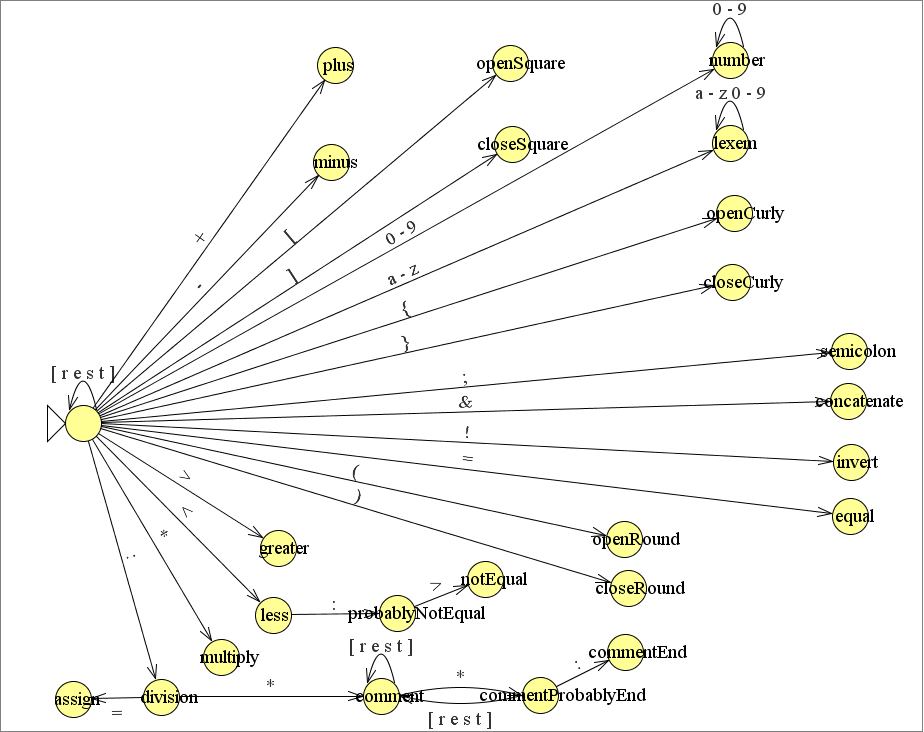
\includegraphics[width=\textwidth]{images/automat}
\label{img:automat}
\caption{Grafische Darstellung des Automaten}
\end{figure}

\subsection{Aufbau des Automaten}
Die Zustandsübergänge sind in Form eines 2D Arrays vorhanden, wobei die 1. Dimension den Ursprungszustand und die 2. Dimension den Zielzustand repräsentiert.
Jedes Zeichen hat in dieser Übergangstabelle einen stellvertretenden Eintrag. Buchstaben sowie Zahlen werden vom Automaten jeweils gruppiert.
Der Startzustand zählt ebenfalls als Rücksetzpunkt, wenn auf einen Zustand mit gegebenen Zeichen kein Folgezustand gefunden wird.
Leerzeichen, Zeilenumbrüche führen in allen Zuständen außer innerhalb von Kommentaren zu einem Übergang zum Rücksetzpunkt.
Unbekannte Zeichen werden innerhalb von Kommentaren akzeptiert, außerhalb von Kommentaren aber als unbekanntes Zeichen repräsentiert.

\subsection{Ablauf}
Für ein eingehendes Zeichen in \verb+int readChar(char c)+ wird zuerst der neue Zustand ermittelt. Dies geschieht intern mit der Methode \verb+nt getNextState(char c)+.
Diese Methode sucht zuerst mittels \verb+int getTransitionColumn(char c)+ den vom aktuellen Zustand abhängigen nächsten Zustand.

Nun wird in \verb+int readChar(char c)+ geprüft, ob dieser neue Zustand nicht der Startzustand ist.

Handelt es sich bei dem neuen Zustand nicht um den Startzustand, dann handelt es sich um einen \glqq validen\grqq\ Übergang im Sinne unserer Grammatik.

\subsubsection{Vorgehen bei validem Übergang}
\verb+lastFinalStateCounter+ wird um eins inkrementiert um den Offset zum letzten validen Zustand zu behalten.
Zudem nimmt der Automat den neuen Zustand an.
Der Automat gibt in diesem Fall den Wert 0 zurück und sagt somit, dass alles in Ordnung ist.

\subsubsection{Vorgehen bei nicht validem Übergang}
Sollte sich der Automat noch in einem finalen Zustand befinden, dann gibt der Automat den aktuellen Zustand zurück und setzt sich wieder auf den Startzustand.
Der Rückgabewert in diesem Fall ist eine positive Zahl und bedeutet somit, dass er einen validen Zustand erreicht hat, bevor er das letzte Zeichen gelesen hat.

Sollte der Automat aber nicht in einem finalen Zustand sein, dann gibt der Automat den negativen \verb+lastFinalStateCounter+ Wert zurück und setzt sich selbst auf den letzten erreichten Finalen Zustand.
Somit gibt der Automat eine negative Zahl zurück, welche die Distanz zum letzten validen Zeichen repräsentiert.


\section{Buffer}\label{sec:buffer}
Die Aufgabe des Buffers ist es die Eingabedatei einzulesen und dem Scanner Zeichen für Zeichen zu übergeben. Dabei soll die Pufferung allein durch das Programm abgewickelt werden, die automatische Pufferung durch das Betriebssystem wird also abgeschaltet. Außerdem muss der Buffer die Möglichkeit bieten Zeichen auch zurückzunehmen. %Vllt Begründung

\subsection{Aufbau}
Der Buffer besteht intern aus zwei unabhängigen Speicherbereichen einer definierten Größe (Buffersize). Bei der Initialisierung wird der erste Speicherbereich mit dem Anfang der Quelldatei gefüllt und bei jedem Lesezugriff auf den Buffer wird der zwischengespeicherte Inhalt der Datei ausgegeben. Falls beim Lesen aus dem Buffer über das Limit des Speicherbereichs hinaus gelesen werden soll, wird der anschließende Bereich in den zweiten Speicherbereich geladen und der Puffer-Zeiger umgesetzt.

Diese Zweiteilung des Buffers hat den Vorteil, dass falls beim Zurücklesen von Zeichen der Anfang des Speicherbereichs überschritten werden würde, nichts aus der Datei geladen werden muss, da der vorherige Teil der Datei noch im zweiten Speicherbereich zwischengespeichert ist und der Zugriff damit direkt erfolgen kann.

\subsection{\od und posix\textunderscore memalign}\label{subsec:odirect}
Um die Pufferung des Betriebssystems zu deaktivieren, muss beim Öffnen der Datei das \verb+O_DIRECT+-Flag gesetzt werden:
\begin{lstlisting}[language=C++]
this->fileDescriptor = open(path, O_RDONLY | O_DIRECT)
\end{lstlisting}

Leider führt die Verwendung von \od häufig zu Problemen. So müssen folgende Vorraussetzungen gegeben sein, damit der \verb+open+-Befehl ohne Fehler abläuft:
\begin{itemize}
\item Verwendung eines Linux-Betriebssystems
\item Die zu öffnende Datei muss auf einer lokalen Festplatte liegen (keine Netzwerkfreigabe o.\,Ä.)
\item Das Betriebssystem darf nicht virtualisiert sein
\end{itemize}

Des Weiteren muss beim Lesen aus einer mit \od geöffneten Datei darauf geachtet werden, dass der Zielbuffer entsprechend ausgerichtet ist und stets nur ein Vielfaches von 512 Bytes gelesen wird.

Bei uns ergibt sich aus diesen Gründen folgende Implementierung für das Öffnen einer Datei, allozieren des Speichers und das Lesen aus der Datei:

\begin{lstlisting}[language=C++,label=lst:bufferinit,caption=Buffer: Initialisierung und Lesen aus Datei]
#define BUFFERSIZE (1024 * (int)sizeof(char))

Buffer::Buffer(const char *path) {
    if ((this->fileDescriptor = open(path, O_RDONLY | O_DIRECT)) < 0) {
		perror("Oeffnen fehlgeschlagen");
		exit(-1);
	}
	// Buffer 1 initialisieren (Platz fuer BUFFERSIZE + 1 chars)
	allocMem(&memptr1, BUFFERSIZE, BUFFERSIZE + sizeof(char));
	// ...
}

// Inline Methode, die Speicher alloziert, nur zur Uebersichtlichkeit ausgelagert.
inline void Buffer::allocMem(void **mempt, int align, int size) {
	if (posix_memalign(mempt, align, size) != 0) {
		perror("Speicher allozieren fehlgeschlagen");
		exit(-1);
	}
}

// Lese count chars in buf, gibt die Anzahl der gelesenen Bytes zurueck
int Buffer::readBytes(char *buf, int count) {
	if (fileDescriptor > 0) {

		int bytesRead = read(this->fileDescriptor, buf, count);

		if (bytesRead < 0) {
			perror("Fehler beim lesen");
			exit(-1);
		}

		// Wenn weniger Bytes zurueckgeliefert wurden als angefordert wurden
		// (Dateiende ist nahe), setze EOF-Markierer hinter letztes gelesenen char
		if (bytesRead < BUFFERSIZE) buf[bytesRead] = '\0';
		return bytesRead;
	}
	return -1; // Falls kein fileDescriptor, sollte nicht auftreten
}
\end{lstlisting}

Da \od am Anfang häufiger zu Problemen führte, wurde es erst eingeschaltet, als der Rest des Buffers implementiert war. Nachdem alle obigen Punkte allerdings erfüllt waren, funktionierte alles wie vorgesehen.

Das folgende Zitat fasst unsere Erfahrungen mit \od auf amüsante Weise erstaunlich gut zusammen:

\begin{quotation}
"'The thing that has always disturbed me about \od is that the whole interface is just stupid, and was probably designed by a deranged monkey on some serious mind-controlling substances."'\\\hspace*{1em}-- Linus Torvalds, aus der \verb+Linux Programmer's Manual+ zu \verb+open(...)+
\end{quotation}

\subsection{Implementierung}
Der Buffer steht, wie oben beschrieben, aus zwei getrennten Speicherbereichen (in diesem Fall: der Größe 1025 Bytes), auf welche, um die Verarbeitung zu vereinfachen, zwei Char-Pointer zeigen. Mit Hilfe dieser Pointer kann über den Arrayzugriffsoperator auf die einzelnen Zeichen zugegriffen werden.
\begin{lstlisting}[language=C++]
return (*this->currentBuffer)[this->currentBufferIndex];
\end{lstlisting}

Das Tauschen der einzelnen Buffer-Teile stellte sich am Ende als keine große Schwierigkeit mehr heraus.

\begin{lstlisting}[language=C++,label=lst:buffertausch,caption=Buffer: Tauschen der Buffer-Teile]
// Pruefung, ob ein neuer Buffer geladen werden muss
if (this->currentBufferIndex < 0) { //Buffer davor laden, BufferIndex wuerde sonst negativ werden
	// Buffer tauschen
	if (this->currentBuffer == &this->buffer1) {
		this->currentBuffer = &this->buffer2;
	} else if (this->currentBuffer == &this->buffer2) {
		this->currentBuffer = &this->buffer1;
	}
	// Index ans Ende des Buffers setzen
	this->currentBufferIndex = BUFFERSIZE-1;
} else if (this->currentBufferIndex >= BUFFERSIZE) { //Naechsten Buffer laden, BufferIndex wuerde sonst ueberlaufen
	if (this->currentBuffer == &this->buffer1) {
		if (!this->memptr2) { // Buffer 2 noch nicht initialisiert
			allocMem(&this->memptr2, BUFFERSIZE, BUFFERSIZE + sizeof(char));
			this->buffer2 = (char*)this->memptr2;
			this->buffer2[BUFFERSIZE] = '\0';
		}
		// Buffer 2 vollladen
		this->readBytes(this->buffer2, BUFFERSIZE);
		// Aktueller Buffer ist Buffer 2
		this->currentBuffer = &this->buffer2;
	} else if (this->currentBuffer == &this->buffer2) {
		// Buffer 1 volladen
		this->readBytes(this->buffer1, BUFFERSIZE);
		// Aktueller Buffer ist Buffer 1
		this->currentBuffer = &this->buffer1;
	}
	// BufferIndex an den Anfang
	this->currentBufferIndex = 0;
}
\end{lstlisting}

\section{Symboltabelle}\label{sec:symtable}
Die Symboltabelle ist eine Sammlung von bekannten Lexemen inklusive ihrer Token. Dabei entspricht die Symboltabelle einer Key-Value-Map mit dem Lexem als Key und dem Token als Value.

\subsection{Implementierung}
Die Symboltabelle ist ein Array mit verketteten Listen. Bei der Initialisierung wird das Array sowie die einzelnen verketteten Listen erstellt.
Die Listen sind zu diesem Zeitpunkt komplett leer.

\subsubsection{Auslesen}
Zum Auslesen wird ein Lexem benötigt. Dieses dient mittels einer Hash-Funktion zur Identifizierung der Konkreten verketteten Liste im Array.
Daraufhin wird innerhalb der verketteten Liste der Eintrag gesucht, der das gleiche Lexem besitzt.

\subsubsection{Einfügen}
Möchte man ein Lexem einfügen, dann wird zusätzlich noch ein TokenType benötigt.
Es wird zuerst geprüft, ob dieses Lexem nicht bereits vorhanden ist und gegebenenfalls die dort hinterlegten Daten zurück gegeben. In diesem Fall wird der mitgegebene TokenType ignoriert.
Ist ein Lexem noch nicht vorhanden, dann wird die Kombination aus Lexem und TokenType in der verketteten Liste gespeichert.

\section{Scanner}\label{sec:scanner_bin}
Der Scanner ist für die Generierung der Tokens anhand einer Datei verantwortlich, von der nur der Pfad bekannt ist. Dazu muss nach der Initialisierung die Methode \verb+nextToken()+ aufgerufen werden.

\subsection{Initialisierung}
Der Scanner benötigt zur Initialisierung den Pfad zu der Quelldatei sowie eine Symboltabelle. Als erstes wird ein neuer Buffer mit dem Pfad zur Quelldatei erstellt sowie ein neuer Automat erstellt.

In die Symboltabelle werden dann die bekannten Schlüsselwörter als entsprechende Token eingetragen.

\subsection{nextToken()}
Diese Methode ist dafür verantwortlich das nächste Token aus der Datei zu generieren.

Dazu wird so lange aus dem Buffer der nächste Buchstabe ausgelesen, wie ein Zeichen ausgelesen wird, welcher zu keinem Token gehört. Diese Zeichen sind die Zeilenumbrüche sowie Whitespaces, wie Tabs oder Leerzeichen. Somit werden diese Zeichen vor einem neuen Token ignoriert.

Als nächstes wird gespeichert, in welcher Zeile und Spalte man sich gerade befindet. Dies ist für Debug Informationen wichtig.

Daraufhin wird innerhalb einer Schleife immer wieder dasselbe getan:
\begin{itemize}

\item Aus dem Buffer wird der nächste Buchstabe ausgelesen. Handelt es sich hierbei um ein \verb+\0+, dann ist die Datei zu Ende. 

\item Im Automaten wird geprüft, in was für einem Zustand man sich befindet und das Ergebnis wird als Token zurück gegeben.

\item Gibt der Buffer kein \verb+\0+, dann wird dieser Buchstabe in den Automaten gegeben. Handelt es sich um einen validen Übergang wird der Automat gefragt, ob das Zeichen gespeichert werden soll. Falls ja, dann wird das Zeichen in einem char Array zwischengespeichert. Dies ist nötig um Lexeme zu speichern.

\item Gibt der Automat keine 0 zurück, dann handelt es sich um einen invaliden Überang. In diesem Fall wird geprüft, ob der Wert positiv oder negativ ist: ist der Wert negativ, dann muss der Buffer die invertierte Anzahl Schritte zurück gehen. Falls der Wert positiv ist, dann muss der Buffer nur einen Schritt zurück gehen. 

\item Der Automat wird nach dem letzten validen Zustand gefragt. 

\item Die zwischengespeicherten Buchstaben werden mit einem \verb+\0+ terminiert und die bekannten Informationen nun zu einem Token zusammen gefasst.

\end{itemize}
\chapter{Parser}\label{kap:parser}
Der Aufgabenteil \emph{Parser} implementiert die Aufgaben der \emph{syntaktischen und semantischen Analyse} unseres Compilers. Das bedeutet, dass der Parser aus den Tokens, die er vom Scanner bekommt einen Strukturbaum aufbauen muss und auf diese Weise überprüft, ob die Ausdrücke in der Eingabedatei entsprechend der Grammatik gültig sind (syntaktische Analyse). Im nächsten Schritt wird überprüft, ob die Ausdrücke auch grundlegend logisch sind (z.\,B. Identifier definiert sind, Rechnungen nur mit gleichen Datentypen durchgeführt werden, etc.). Dieser Schritt wird semantische Analyse genannt.

Um diese Aufgaben erfüllen zu können, besteht der Parser aus zwei Teilen:
\begin{itemize}
\item dem Parse-Tree, welcher die Regeln unserer Grammatik in Programmstrukturen (Interfaces und Klassen) darstellt, und 
\item dem Parser selbst, welcher die Tokens entgegennimmt und prüft, welche Tokens wann gültig sind und welche Knoten am Baum angehängt werden. Der Parser baut auch den Strukturbaum selbst auf.
\end{itemize}

\section{Parse-Tree}\label{sec:parsetree}
In unserer Implementierung ist die Struktur des Baumes sehr umfangreich, da wir die zweite in den Folien genannte Alternative implementiert haben, welche daraus besteht für jede einzelne Regel der Grammatik eine eigene Klasse zu erstellen und für jedes Nichtterminal ein Interface, welches die einzelnen Regeln implementieren müssen. Diese Variante hat den großen Vorteil, dass man den Strukturbaum nicht invalide aufbauen kann, da nur vorher festgelegte Klassen, entsprechend der Grammatik, angehängt werden können. So können z.\,B. an einen \verb+STATEMENTS+-Knoten nur ein \verb+STATEMENT+ sowie ein \verb+STATEMENTS+-Knoten angehängt werden; andere Konstellationen sind nicht möglich.

Alle Knoten erben außerdem vom \verb+IParseTree+-Interface, welches die grundlegenden Methoden, die jede Klasse implementieren muss vorschreibt:

\begin{lstlisting}[language=C++,label=lst:parsetree,caption=Parser: IParseTree-Interface]
class IParseTree {
private:
    int line, col;
public:
    virtual void typeCheck(Symboltable *symtable)=0;
    virtual void makeCode(std::ofstream *code)=0;
    Type type;
    void setPos(int line, int col){this->line = line; this->col = col;};
    int getLine(){return this->line;};
    int getCol(){return this->col;};
};
\end{lstlisting}

Die Klassenstruktur einer einzelnen Regeln sieht, hier am Beispiel der Regel Decl\textunderscore I (\verb+int ARRAY identifier+, wobei \verb+int+ ein Terminal (Schlüsselwort) ist), wie folgt aus:

\begin{lstlisting}[language=C++,label=lst:decl_i,caption=Parser: Klassenstruktur von Decl\textunderscore I]
class Decl_I : public IDecl { // Decl_I implmentiert das Interface IDecl
public:
    Decl_I(const char *identifier); // Im Konstruktor wird der Identifier uebergeben
    virtual ~Decl_I();
    void typeCheck(Symboltable *symtable);
    void makeCode(std::ofstream *code);
    void addNodes(IArray *array); // Es darf nur ein Knoten vom Typ IArray angehaengt werden
private:
    IArray *array;
    const char *identifier;
};
\end{lstlisting}

\subsection{Type-Check}
Der Type-Check dient der semantischen Analyse des aufgebauten Strukturbaumes. Er wird am Ursprungsknoten gestartet und läuft dann rekursiv jeden einzelnen Knoten des Baumes ab, bis alle Knoten geprüft sind. Falls bei der Überprüfung ein Fehler gefunden wird (z.\,B. die Verwendung eines unbekannten Identifiers), wird eine Fehlermeldung ausgegeben, der Vorgang aber nicht komplett abgebrochen, da ein Fehler hier zwar ein logischer Fehler ist, der Erzeugung des Codes aber nicht im Wege steht (ein Fehler würde erst bei der Ausführung des Codes auftreten). Ein Abbruch des Programms ist aber möglich und auch theoretisch vorgesehen, es muss nur eine Zeile einkommentiert werden.

Für den Type-Check musste auch die Symboltabelle angepasst werden. Die Möglichkeit zu einem Identifier den Typ abzuspeichern, welchen dieser Identifier beschreibt (z.\,B. Integer oder Array) war vorher nicht vorgesehen und wurde eingefügt. Dazu wurden die Methoden \verb+storeIdentifierType()+ und \verb+getIdentifierType()+ implementiert, welche einfach noch ein weiteres Feld zum Identifier speichern.

\subsection{Code-Erzeugung}
Die Aufgabe der Code-Erzeugung wird in den einzelnen Klassen durch die Methode \verb+makeCode()+ implementiert. Auch hier wird der Baum rekursiv durchlaufen, jeder Knoten muss also auch die Code-Erzeugung bei seinen Kind-Knoten aufrufen. Als Beispiel hier die Code-Erzeugung bei \verb+Statement_I+, also der Regel \verb+identifier INDEX := EXP+, welche die Zuweisung einer Variablen darstellt:

\begin{lstlisting}[language=C++,label=lst:makecodestatementi,caption=Parser: Code-Erzeugung des Zuweisung-Statements]
void Statement_I::makeCode(std::ofstream *code) {
    this->exp->makeCode(code); // Rufe Code-Erzeugung beim Child-Node exp auf
    *code << "LA " << "$" << this->identifier << ENDL; // Fuege "Lade-Adresse" des Identifiers ein
    this->index->makeCode(code); // Falls ein Array-Zugriff erfolgen soll, fuege diesen Zugriff ein
    *code << "STR" << ENDL; // Fuege den "Store"-Befehl ein
}
\end{lstlisting}

\subsubsection{Besonderheiten bei '>' und '<:>'}
Da es in der Assembler-Sprache die Konstrukte \glqq größer als\grqq\ und \glqq ungleich\grqq\ nicht gibt, diese aber in unserer Grammatik vorgesehen sind müssen diese in valide, gleichbedeutende Ausdrücke umgewandelt werden.

So wird, nach folgender Formel, im Falle von \glqq größer als\grqq\ einfach ein \glqq kleiner als\grqq\ verwendet und die beiden Operanden getauscht:

$a > b \iff b < a$

Im Falle von \glqq ungleich\grqq\ ist es ähnlich einfach: hier wird das \glqq ungleich\grqq\ durch ein \glqq gleich\grqq\ ersetzt und das Ergebnis am Ende negiert:

$a \neq b \iff \neg(a = b)$

\section{Parser}\label{sec:parser_bin}
Der Parser selbst hat neben der \verb+parse()+-Methode, welche den Parse-Vorgang startet und einer Methode, die Labels generiert, für jedes Nichtterminal eine Methode, welche den Baum unterhalb dieses Nichtterminals rekursiv aufbaut. Der Aufruf muss hier also auch nur einmal, an der Wurzel, erfolgen und der komplette Strukturbaum entsteht automatisch.

Die Methode \verb+parse()+ ist wie folgt implementiert:

\begin{lstlisting}[language=C++,label=lst:parser_parse,caption=Parser: Methode parse()]
void Parser::parse(const char *path) {
	// Ausgabedatei oeffnen
    std::ofstream code(path, std::ios::out | std::ios::trunc);

    // Erstes Token anfordern
    nextToken();

    printf("parsing...\n");
    // Baum aufbauen, Wurzel ist immer ein PROG
    IParseTree *parseTree = PROG();
    
    printf("type checking...\n");
    // Type-Check an der Wurzel starten
    parseTree->typeCheck(this->symtable);
    
    printf("generating code...\n");
    // Code-Erzeugung an der Wurzel starten
    parseTree->makeCode(&code);
    printf("stop.\n");

    code.close();
}
\end{lstlisting}

Als Beispiel für das Aufbauen des Baumes hier die Methode \verb+DECL()+:

\begin{lstlisting}[language=C++,label=lst:decl,caption=Parser: Methode DECL()]
IDecl* Parser::DECL() {
    IDecl *tree;
    if (currentToken->getTokenType() == tokenInt) {
        nextToken();
        IArray *array = ARRAY();
        if (currentToken->getTokenType() == tokenIdentifier) {
            tree = new Decl_I(currentToken->getInformation()->getLexem());
            tree->setPos();
            static_cast<Decl_I*>(tree)->addNodes(array);
            nextToken();
        } else {
            error("expected identifier", currentToken);
        }
    } else {
        error("unidentified token", currentToken);
    }
    return tree;
}
\end{lstlisting}
Da die Methode \verb+addNodes()+ bei jeder Klasse unterschiedliche Parameter erfordert, kann diese weder bei den Nichtterminal-Interfaces, noch beim Parse-Tree-Interface vorgeschrieben sein. Damit der Aufruf erfolgen kann, muss das Objekt \verb+tree+, vom Typ \verb+IDecl+ für diesen Aufruf in ein Objekt vom Typ \verb+Decl_I+ gecastet werden. Dies ist problemlos möglich, da \verb+tree+ tatsächlich ein Objekt vom Typ \verb+Decl_I+ ist und erfolgt überall dort, wo die Methode \verb+addNodes+ aufgerufen wird.

Die \verb+error+-Methode gibt eine Fehlermeldung, mit Angabe von Zeile und Spalte aus und beendet das Programm.

Für die Konstrukte \verb+if+ und \verb+while+ der Grammatik, werden Labels benötigt, welche im Programm eindeutig sein müssen. Für die Erzeugung der Labels implementiert der Parser eine Methode, welche bei jedem Aufruf einen Integer hochzählt und zurückgibt. In der Code-Erzeugung, wo die Labels benötigt werden, wird diesem Integer ein Rautensymbol (kennzeichnet ein Label), sowie ein \glqq L\grqq\ zuvorgestellt, denn ein Label muss genau so aufgebaut sein, wie ein Identifier, darf also nicht mit einer Ziffer beginnen. Auf diese Variante ist die Erzeugung der Labels relativ einfach und die Eindeutigkeit garantiert.

\begin{figure}[b]
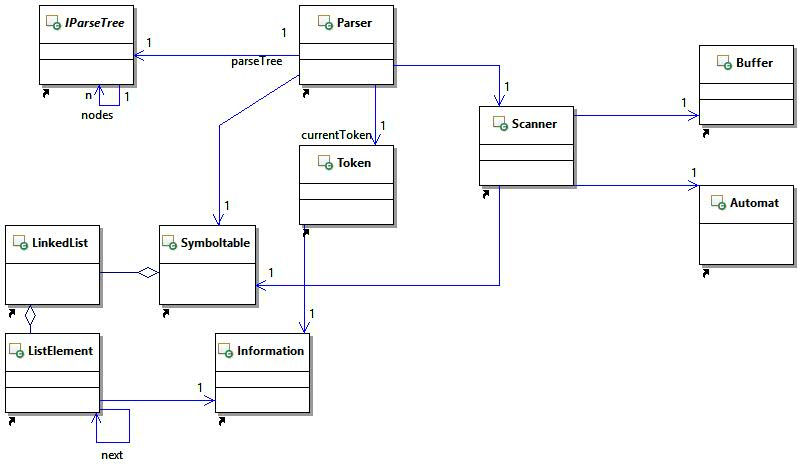
\includegraphics[width=\linewidth]{images/klassendia2}
\label{img:klassendia}
\caption{Klassendiagramm des Compilers}
\end{figure}

\end{document}
